%%%%%%%%%%%%%%%%%%%%%%%%%%%%%%%%%%%%%%%%%%%%%%%%%%%%%%%%%%%%%%%%%%%%%%%%%%%%%%%%
%2345678901234567890123456789012345678901234567890123456789012345678901234567890
%        1         2         3         4         5         6         7         8

%\documentclass[letterpaper, 10 pt, conference]{ieeeconf}  % Comment this line out
% if you need a4paper
\documentclass[a4paper, 10pt, conference]{ieeeconf}      % Use this line for a4
% paper



% The following packages can be found on http:\\www.ctan.org
\usepackage{graphics} % for pdf, bitmapped graphics files
\usepackage{epsfig} % for postscript graphics files
%\usepackage{mathptmx} % assumes new font selection scheme installed
%\usepackage{times} % assumes new font selection scheme installed
%\usepackage{amsmath} % assumes amsmath package installed
%\usepackage{amssymb}  % assumes amsmath package installed

\title{\LARGE \bf
	Testing the Performance of Linear Regressors Using Inertial Information Combined with sEMG to Minimize the Limb Position Effect in Proportional and Simultaneous Control of Lower Arm Prosthetics.
}%final name

%\author{ \parbox{3 in}{\centering Huibert Kwakernaak*
%         \thanks{*Use the $\backslash$thanks command to put information here}\\
%         Faculty of Electrical Engineering, Mathematics and Computer Science\\
%         University of Twente\\
%         7500 AE Enschede, The Netherlands\\
%         {\tt\small h.kwakernaak@autsubmit.com}}
%         \hspace*{ 0.5 in}
%         \parbox{3 in}{ \centering Pradeep Misra**
%         \thanks{**The footnote marks may be inserted manually}\\
%        Department of Electrical Engineering \\
%         Wright State University\\
%         Dayton, OH 45435, USA\\
%         {\tt\small pmisra@cs.wright.edu}}
%}

\author{Simon Bruun, Oliver Thomsen Damsgaard, Martin Alexander Garenfeld, Irene Uriarte}% <-this % stops a space


\begin{document}
	
	
	
	\maketitle
	\thispagestyle{empty}
	\pagestyle{empty}
	
	
	%%%%%%%%%%%%%%%%%%%%%%%%%%%%%%%%%%%%%%%%%%%%%%%%%%%%%%%%%%%%%%%%%%%%%%%%%%%%%%%%
	\begin{abstract}
Electromyography (EMG) is widely used as input to control scheme of myoelectric prosthetics. However, EMG signals change with limb position and this lowers the accuracy in classification. Inclusion of Inertial Measurement Units (IMU) has proved to raise the accuracy in pattern recognition methods. However, pattern recognition methods provides only control of one degree of freedom (DoF) at a time. This study propose to use a combination of EMG recordings and accelerometer data in a linear regression model to enable a simultaneous and proportional control scheme. In this study recordings from four(more now)  able-bodied subjects has been collected, performing flexion, extension, radial and ulnar deviation of the wrist in three different limb positions. The data was evaluated through principal component analysis (PCA) and processed/trained with a linear regression model to classify the hand movements. One regressor is trained for each wrist movement, using EMG data as well as a combination of EMG and IMU data. The regressors are tested in a real-time visual environment on PC, measuring time to complete a target-reaching task of sixteen targets. The performance of the regressors are compared when the IMU data is added to the training process and when is not, to determine the effect of it. 
	
	\end{abstract}
	
	
	%%%%%%%%%%%%%%%%%%%%%%%%%%%%%%%%%%%%%%%%%%%%%%%%%%%%%%%%%%%%%%%%%%%%%%%%%%%%%%%%
	\section{INTRODUCTION}
In recent years the development of EMG controlled prosthesis have advanced due to an increased interest in the area as well as a higher demand of better control of this prosthesis.\cite{fougner2012}
In the early years most EMG prosthetics functioned by only controlling one DOF by \textit{on-off control}, mostly by linking antagonistic muscles to one DOF. This along with \textit{mode switching} provided users a way to control more than one DOF, but not in a simultaneous way. However, as demands would rise, more complex methods was introduced to the EMG scene, and proportional control was brought in with pattern recognition methods. This effectively enabled simultaneous control of more than one DOF, but gave rise to new problems; a wider range of control would give less accurate movements, and training the pattern recognition methods proved difficult, as the training could over-fit, causing extended use of the prosthetics to degrade in performance. \cite{Ison2016}. It has been proved that regression techniques can be apply as a new mapping method to achieve simultaneous and proportional control of multiple DOFs\cite{hanhe2014}. However there are still difficulties when prosthesis perform outside the clinical training environment\cite{jiang2012}. Fougner et al.\cite{Fougner2011} noticed that majority of studies only take in account one limb position which becomes a problem since muscles create muscle-synergies to perform movements. It has been demonstrated that the variations in limb positions can have an impact on the robustness of EMG pattern recognition. To be able to offer a good perform of the prosthesis, these should be able to execute with the same accuracy diverse hand gestures in different limb positions. In order to overcome this problem it has been suggested to combine EMG data as well as IMU data in the training sesions of the regressor to obtain simultaneous and proportional control of EMG prosthesis. 
%Hypotheses
Simultaneous and proportional control of two  DOF's of the wrist in different limb positions, can be achieve trough the use of linear regression as control system. Combining EMG and IMU's can minimize the limb position effect when using regression as control system.	

	\section{METHODS}
	
	\subsection{Experimental Setup}
EMG data was collected from four able-bodied subjects. The subjects performed four different hand gestures. This study is only focus on two DOF, which are, flexion, extension, radial and ulnar deviation of the wrist. The order in the execution of the movements was the same for each subject. EMG signals were recorded with Myo armband, positioned in the right forearm of the subjects (all subjects right handed). The procedure was performed in three different limb positions. In order to avoid shoulder fatigue a relaxation period was given between trials. The subjects were instructed not to move the fingers during the data acquisition. The process was performed in a standing position. \\ %figure hand and limb positions
 Myo armband counts with eight medical grade stainless steel surface EMG sensors. %It is capable of pulling EMG data at a sample rate of 200 Hz. 
 Furthermore its nine axis IMU provides information about position and orientation of the arm combining three axis accelerometer, three axis gyroscope and three axis magnetometer. In order to acquire the training data necessary to build the regressor, a graphical user interface (GUI) was implemented in MATLAB. Firstly baseline was meassure holding the forearm relaxed and the wrist in a neutral position for the corresponding limb position. This measure was substracted from the signal afterwards to be able to remove the present artefacts. Subsequently maximum voluntary contraction (MVC) was meassure. The MVC  was calculated as a mean of the maximum values in each of the eight cannels, and was set as a normalized reference point of 1.
 The data acquisition was depicted through a trapeze. MVC was set as the desired value before data acquisition. Consequently each hand gesture was performed as a fraction of the MVC. At the begining of the training data collection two second resting phase was given followed by two seconds ascending slope to reach the plateau phase, with a duration of three seconds. Afterwards a descending phase of two seconds and a resting phase of one second finalized the data acquisition. The total acquisition time was ten seconds per hand movement.


	
	%\subsection{Maintaining the Integrity of the Specifications}
	
	%The template is used to format your paper and style the text. All margins, column widths, line spaces, and text fonts are prescribed; please do not alter them. You may note peculiarities. For example, the head margin in this template measures proportionately more than is customary. This measurement and others are deliberate, using specifications that anticipate your paper as one part of the entire proceedings, and not as an independent document. Please do not revise any of the current designations
	
	\subsection{Preprocessing}
	For this study the EMG data acquired were filtered using a second-order Butterworth high-pass filter, cutoff frequency ($f_c$=10Hz), to avoid low frequency movement artefacts in the recorded signal.\\
	%review two states part trapeze!!
	The EMG signal is the result of the addition of different motor unit action potential trains (MUAPTs). Through the data acquisition phase EMG signal can be divided into two main states. The transient state, related with the beginning phase of the muscle contraction and the steady state which is the stable phase of the muscle contraction when a constant position is held \cite{mobarak2014}. Although the steady state only contains a short temporal structure of the patterns involved in the contraction of the muscle \cite{mobarakm2014}, studies has shown that it is possible to achieve online continuous control using steady state EMG signals.This could be due to the fact that a larger amount of meaningful data is contained in this muscle contraction phase \cite{mobarakm2014}. For the training of the control system in this project the steady signal was then used.
	
	\subsection{Feature extraction}
	The features were extracted creating a sliding-window of 40 samples. % with an overlapping of the 50\%. 
	Two different time domain features were extracted, Mean absolute value (MAV) as well as logarithmic variance. MAV represent the amplitud of the signal. It is defined as the average of the absolute values of the EMG signal and expresed as:
	\begin{equation}
	MAV = \frac{1}{N}\sum\limits_{i=1}^N|x_i|
	\end{equation}
	where N is the length of the signal, and $x_i$ is the signal of $i$ samples.
	The logarithmic variance is a nonlinear transformation of the variance applied to %linealidad
	\begin{equation} \label{eq:logvar}
	log(\sigma^2) = log(\frac{\sum\limits_{i=1}^N(x_i - \mu)^2}{N})
	\end{equation}
	where N expresses the length of the signal, $x_i$ is the $i^th$ sample of the signal and $\mu$ is the mean.
	\subsection{Separability of data}
	In order to evaluate the quality of the features extracted from the EMG signals, Principal Component Analysis (PCA) was applied. This analysis tool express a set of correlated variables into non-correlated components. In that way, the data set can be expressed in a reduced dimensionality hyperspace using less but most representative variables which are the principal components. Through PCA is  possible to see significant outliers or if the clusters formed by the features can be easily distinguishable. This was done to avoid inaccurate training of the regressors. PCA was performed for each movement in each limb position. %and represented in three dimensional space.figure? 
	\subsection{Regression models}
	The acquired data was used to train the four different regressors that had been implemented, one for each movement under study. Simple linear regression had been applied as is shown in \ref{reg}:
	\begin{equation} \label{eq:simpleLinearRegression}
	Y_i = \alpha + \beta X_i + \epsilon_i
	\label{reg}
	\end{equation}
	where, $Y$ is the dependent variable or response, $X$ is the independent variable or the predictor, $\beta$ is the regression coefficient or the slope, and $\alpha$ is the Y intercept (predicted value of $Y$ at $X = 0$),  $\epsilon$ is the error and $i$ is the index.
	
	
	\subsection{Regressor accuracy}
	Superimposition\\
	%To examine the performance of the regressors the estimations of the linear regressor and the true labels for the two different features extracted had been superimposed. Thereby the behave of the regressor can be shown at different intensities and movements. Consequently whether other regression methods should be considered to obtain a lower error.\\
	RMSE\\
	To meassure the accuracy of the regressor, Root Mean Squared Error (RMSE) was calculated. RMSE is a calculation of the standard deviation of the residuals, that is, the difference between the estimated and the actual values.
	%equation
	\begin{equation}
	RMSE = \sqrt{\frac{\sum\limits_{i=1}^N(y_i - \hat{y_i})^2}{N}}
	\end{equation}
	Where N is the length of the signal, $y_i$ is the $i^th$ variable of the actual data and $\hat{y_i}$ is the $i^th$ output of the regressor. The RMSE will be done for the regressor of each movement.\\
	
	Fitts Law\\
	A modified version of Fitts' Law had been used to quantify the performance of the trained regressors. Fitts' Law describes that, the time it takes to do a rapid movement to reach a target area, is dependent on the distance to the target area, and the size of the target area. The law demonstrates that the information of any human motor tasks, is finite and only limited by the capabilities of the control system. The control exhibit a negative correlation between speed and accuracy. \cite{Kamavuako2014}
	Fitts' Law calculates an \textit{Index of Difficulty} (ID) by \ref{eq:Fitts}
	
	\begin{equation} \label{eq:Fitts}
	ID = log_{2} \cdot (\frac{2D}{W})
	\end{equation}
	
	where D is distance to the targets and W is width of target area. The system in this study does not provide a reasonable scale for distance and target width, for this reason Fitts' Law cannot be apply as usual. Instead, the time it takes a subject to reach the targets as well as the number of targets reached will be noted to calculate a performance score as shown in \ref{eq:ourScore}.
	
	\begin{equation} \label{eq:ourScore}
	Score = \frac{time}{targets\ reached}
	\end{equation}
	Consequently low score results represent the best performance.
	To accomplish the modified Fitts' Law test a compass-plot was implemented in the GUI Fig.\ref{figurelabel}. The subjects had to reach 16 targets distributed around the origin in two different radius. This allows to test the proportional control. The targets were fixed in the diagonals of the compass-plot to be able to test simultaneous control. The amount of targets reached in each quadrant gives important information about the regressor performance as well as, providing the weak directions.
	\begin{figure}[thpb]
		\centering
		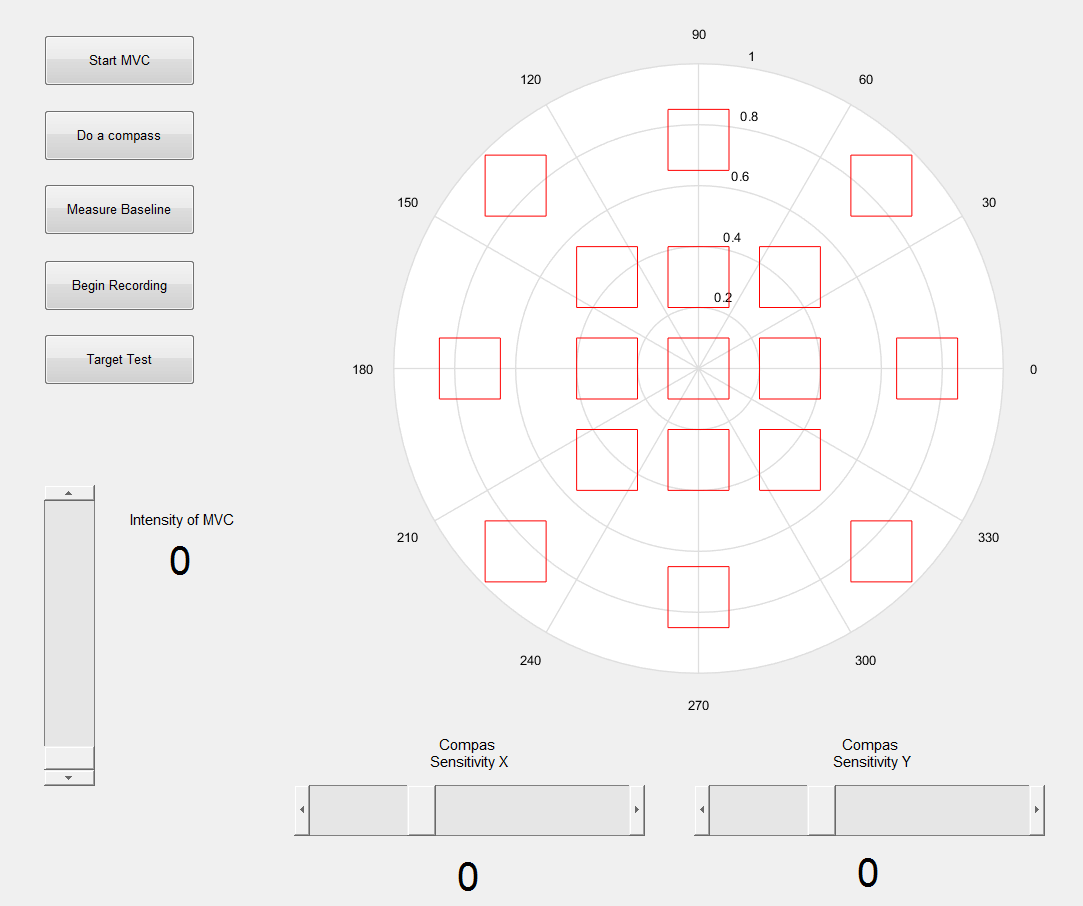
\includegraphics[scale=.2]{Figures/PlacesToGo}
		\caption{GUI}
		\label{figurelabel}
	\end{figure}
	

	
	\section{RESULTS}
	
	something!!! 
	
	\subsection{Separability of the data} 
	PCA performance for both features extracted is illustrated in Fig. \ref{PCA_MVA} (MVA) and in Fig. \ref{PCA_logvar} (logarithmic variance).
	The importance of each component for MAV and logarithmic variance is represented in Fig. \ref{PCA_MVA}(a) and Fig. \ref{PCA_logvar}(a) respectively. On the one hand for the MAV feature making use of the three first components, 93.8\% of the data set can be described. On the other hand for the logarithmic variance feature the 93.97\% of the data set is describe with the three first components. This three PC have been plot for both features Fig. \ref{PCA_MVA}(b) and Fig. \ref{PCA_logvar}(b). There is no presence of remarkable outliers on two data sets and the formed clusters are easily distinguishable.


	\subsection{Regression accuracy} 
Through a quantitative examination of the figure(figure),is observed that MAV performed slightly better than the logarithmic variance for low intensities. However, both estimates yielded inaccurate fitting in high intensities, especially for ulnar deviation of the wrist. It has been extracted from the results illustrated in (figure), which represent the RMSE of the four different regressos for both features of the training data, than $RMSE_{MAV}$= 0.0867$\pm 0.031$ and $RMSE_{logvar}$= 0.1047$\pm 0.0273$. Overall MAV provided a lower mean but a higher standard deviation compared with logarithmic variance.

		\begin{figure}[thpb]
		\centering
		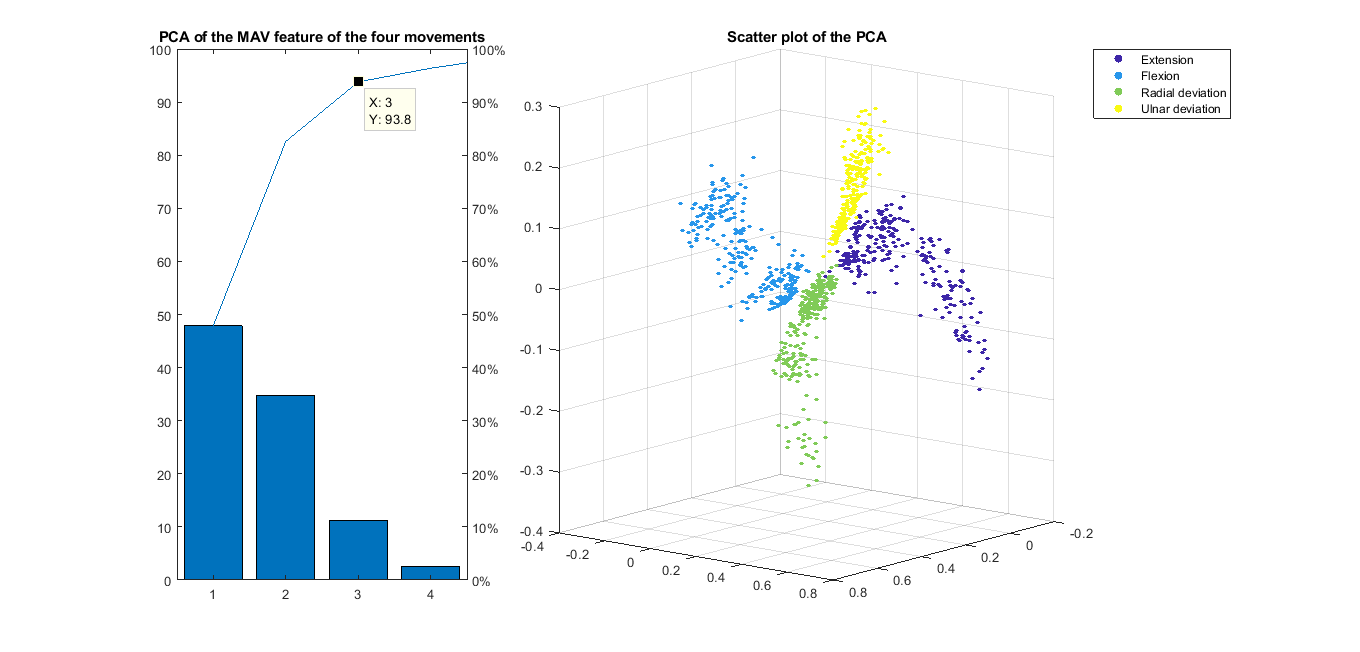
\includegraphics[scale=.27]{Figures/pcasubplotMAV}
		\caption{Inductance of oscillation winding on amorphous
			magnetic core versus DC bias magnetic field}
		\label{PCA_MVA}
	\end{figure}

\begin{figure}[thpb]
	\centering
	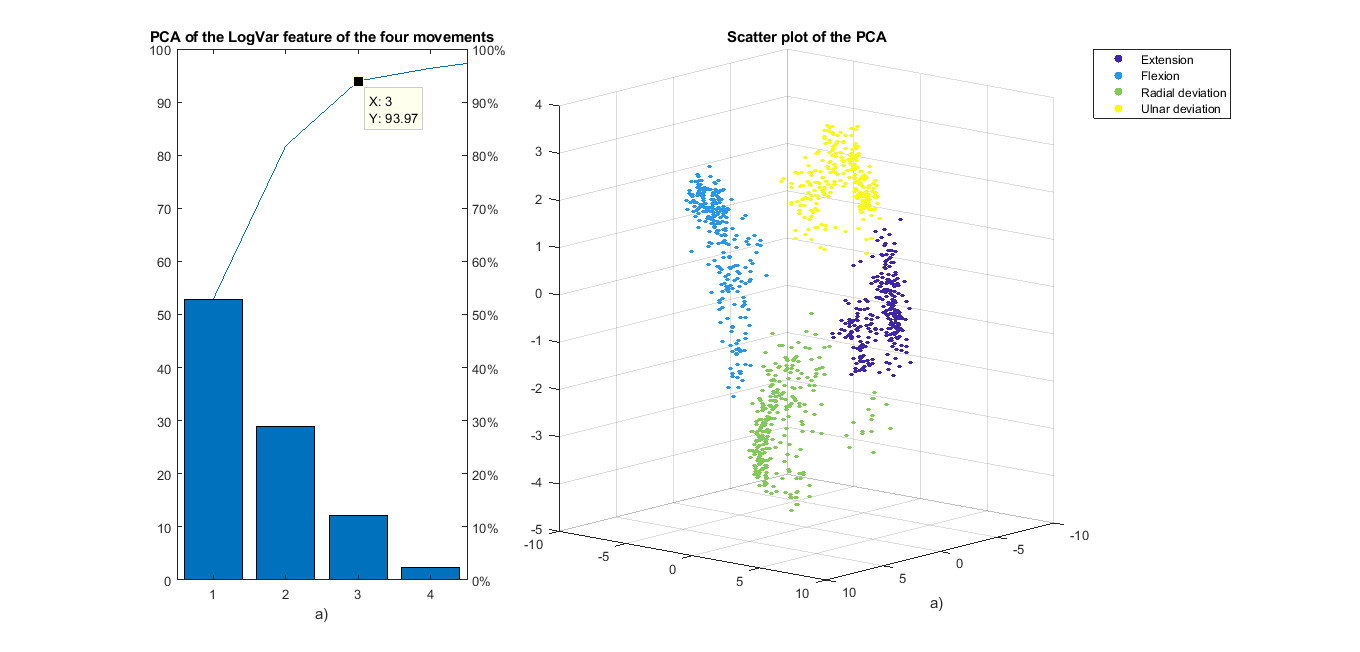
\includegraphics[scale=.27]{Figures/pcasubplotLogVar}
	\caption{Inductance of oscillation winding on amorphous
		magnetic core versus DC bias magnetic field}
	\label{PCA_logvar}
\end{figure}
	\section{DISCUSSION}
	
	
	
%	\begin{table}[h]
%		\caption{An Example of a Table}
%		\label{table_example}
%		\begin{center}
%			\begin{tabular}{|c||c|}
%				\hline
%				One & Two\\
%				\hline
%				Three & Four\\
%				\hline
%			\end{tabular}
%		\end{center}
%	\end{table}
	


	
	
	Figure Labels: Use 8 point Times New Roman for Figure labels. Use words rather than symbols or abbreviations when writing Figure axis labels to avoid confusing the reader. As an example, write the quantity ÒMagnetizationÓ, or ÒMagnetization, MÓ, not just ÒMÓ. If including units in the label, present them within parentheses. Do not label axes only with units. In the example, write ÒMagnetization (A/m)Ó or ÒMagnetization {A[m(1)]}Ó, not just ÒA/mÓ. Do not label axes with a ratio of quantities and units. For example, write ÒTemperature (K)Ó, not ÒTemperature/K.Ó
	
	\section{CONCLUSIONS}
	
 Linear regression methods were applied for the two different features extracted. We compared both performance, training the regressor with EMG data as well as a combination of EMG data and IMU data.
	
	\addtolength{\textheight}{-12cm}   % This command serves to balance the column lengths
	% on the last page of the document manually. It shortens
	% the textheight of the last page by a suitable amount.
	% This command does not take effect until the next page
	% so it should come on the page before the last. Make
	% sure that you do not shorten the textheight too much.
	
	%%%%%%%%%%%%%%%%%%%%%%%%%%%%%%%%%%%%%%%%%%%%%%%%%%%%%%%%%%%%%%%%%%%%%%%%%%%%%%%%
	
	
	
	%%%%%%%%%%%%%%%%%%%%%%%%%%%%%%%%%%%%%%%%%%%%%%%%%%%%%%%%%%%%%%%%%%%%%%%%%%%%%%%%
	
	
	
	%%%%%%%%%%%%%%%%%%%%%%%%%%%%%%%%%%%%%%%%%%%%%%%%%%%%%%%%%%%%%%%%%%%%%%%%%%%%%%%%
	\section*{APPENDIX}
	
	Appendixes should appear before the acknowledgment.
	
	\section*{ACKNOWLEDGMENT}
	
	The preferred spelling of the word ÒacknowledgmentÓ in America is without an ÒeÓ after the ÒgÓ. Avoid the stilted expression, ÒOne of us (R. B. G.) thanks . . .Ó  Instead, try ÒR. B. G. thanksÓ. Put sponsor acknowledgments in the unnumbered footnote on the first page.
	
	
	
	%%%%%%%%%%%%%%%%%%%%%%%%%%%%%%%%%%%%%%%%%%%%%%%%%%%%%%%%%%%%%%%%%%%%%%%%%%%%%%%%
	
	References are important to the reader; therefore, each citation must be complete and correct. If at all possible, references should be commonly available publications.
	
	
	
	\begin{thebibliography}{99}
		
		\bibitem{c1} G. O. Young, ÒSynthetic structure of industrial plastics (Book style with paper title and editor),Ó 	in Plastics, 2nd ed. vol. 3, J. Peters, Ed.  New York: McGraw-Hill, 1964, pp. 15Ð64.
		\bibitem{c2} W.-K. Chen, Linear Networks and Systems (Book style).	Belmont, CA: Wadsworth, 1993, pp. 123Ð135.
		\bibitem{c3} H. Poor, An Introduction to Signal Detection and Estimation.   New York: Springer-Verlag, 1985, ch. 4.
		\bibitem{c4} B. Smith, ÒAn approach to graphs of linear forms (Unpublished work style),Ó unpublished.
		\bibitem{c5} E. H. Miller, ÒA note on reflector arrays (Periodical styleÑAccepted for publication),Ó IEEE Trans. Antennas Propagat., to be publised.
		\bibitem{c6} J. Wang, ÒFundamentals of erbium-doped fiber amplifiers arrays (Periodical styleÑSubmitted for publication),Ó IEEE J. Quantum Electron., submitted for publication.
		\bibitem{c7} C. J. Kaufman, Rocky Mountain Research Lab., Boulder, CO, private communication, May 1995.
		\bibitem{c8} Y. Yorozu, M. Hirano, K. Oka, and Y. Tagawa, ÒElectron spectroscopy studies on magneto-optical media and plastic substrate interfaces(Translation Journals style),Ó IEEE Transl. J. Magn.Jpn., vol. 2, Aug. 1987, pp. 740Ð741 [Dig. 9th Annu. Conf. Magnetics Japan, 1982, p. 301].
		\bibitem{c9} M. Young, The Techincal Writers Handbook.  Mill Valley, CA: University Science, 1989.
		\bibitem{c10} J. U. Duncombe, ÒInfrared navigationÑPart I: An assessment of feasibility (Periodical style),Ó IEEE Trans. Electron Devices, vol. ED-11, pp. 34Ð39, Jan. 1959.
		\bibitem{c11} S. Chen, B. Mulgrew, and P. M. Grant, ÒA clustering technique for digital communications channel equalization using radial basis function networks,Ó IEEE Trans. Neural Networks, vol. 4, pp. 570Ð578, July 1993.
		\bibitem{c12} R. W. Lucky, ÒAutomatic equalization for digital communication,Ó Bell Syst. Tech. J., vol. 44, no. 4, pp. 547Ð588, Apr. 1965.
		\bibitem{c13} S. P. Bingulac, ÒOn the compatibility of adaptive controllers (Published Conference Proceedings style),Ó in Proc. 4th Annu. Allerton Conf. Circuits and Systems Theory, New York, 1994, pp. 8Ð16.
		\bibitem{c14} G. R. Faulhaber, ÒDesign of service systems with priority reservation,Ó in Conf. Rec. 1995 IEEE Int. Conf. Communications, pp. 3Ð8.
		\bibitem{c15} W. D. Doyle, ÒMagnetization reversal in films with biaxial anisotropy,Ó in 1987 Proc. INTERMAG Conf., pp. 2.2-1Ð2.2-6.
		\bibitem{c16} G. W. Juette and L. E. Zeffanella, ÒRadio noise currents n short sections on bundle conductors (Presented Conference Paper style),Ó presented at the IEEE Summer power Meeting, Dallas, TX, June 22Ð27, 1990, Paper 90 SM 690-0 PWRS.
		\bibitem{c17} J. G. Kreifeldt, ÒAn analysis of surface-detected EMG as an amplitude-modulated noise,Ó presented at the 1989 Int. Conf. Medicine and Biological Engineering, Chicago, IL.
		\bibitem{c18} J. Williams, ÒNarrow-band analyzer (Thesis or Dissertation style),Ó Ph.D. dissertation, Dept. Elect. Eng., Harvard Univ., Cambridge, MA, 1993. 
		\bibitem{c19} N. Kawasaki, ÒParametric study of thermal and chemical nonequilibrium nozzle flow,Ó M.S. thesis, Dept. Electron. Eng., Osaka Univ., Osaka, Japan, 1993.
		\bibitem{c20} J. P. Wilkinson, ÒNonlinear resonant circuit devices (Patent style),Ó U.S. Patent 3 624 12, July 16, 1990. 
		
		
		
		
		
		
	\end{thebibliography}
	
	
	
	
\end{document}